\documentclass[a4paper]{article}
\usepackage[a4paper,margin=0mm]{geometry}
\usepackage{fontspec}
\usepackage{unicode-math}
\usepackage{tikz}
\usepackage[table]{xcolor}
\usepackage[absolute]{textpos}
\usepackage{enumitem}
\usepackage{array}
\usepackage{multirow}

\setmainfont{Libertinus Serif}
\setsansfont{Libertinus Sans}
\setmathfont{Libertinus Math}
\newfontfamily\trackedsans{Libertinus Sans}[LetterSpace=8.0]

\definecolor{accent}{HTML}{F46530}
\definecolor{badge}{HTML}{FFBDA5}
\definecolor{ink}{HTML}{2A2E30}

\setlength{\TPHorizModule}{1mm}
\setlength{\TPVertModule}{1mm}
\setlength{\parindent}{0pt}
\pagestyle{empty}

\newcommand{\LCOL}{16mm}
\newcommand{\RCOL}{111mm}
\newcommand{\COLW}{83mm}

\newcommand{\topicheader}[2]{%
\begin{textblock*}{194mm}(16mm,10mm)
\begin{tikzpicture}
\node[fill=accent,text=white,font=\sffamily\bfseries\fontsize{13}{13}\selectfont,
      minimum width=9mm,minimum height=9mm,inner sep=0pt] at (4.5mm,-4.5mm) {#1};
\node[font=\sffamily\bfseries\fontsize{15}{16}\selectfont,text=ink,anchor=west] at (12mm,-4.5mm) {#2};
\end{tikzpicture}
\end{textblock*}
\begin{textblock*}{194mm}(16mm,22.5mm)

\begin{tikzpicture}
\fill[accent] (0,0) rectangle (194mm,0.5mm);
\end{tikzpicture}
\end{textblock*}
}

\newcommand{\pagefooter}[1]{%
\begin{textblock*}{194mm}(8mm,286.41mm)
  
\begin{tikzpicture}
    \fill[accent] (0,0) rectangle (194mm,0.6mm);
  \end{tikzpicture}
\end{textblock*}
\begin{textblock*}{63.59mm}(8mm,288.27mm)
  {\sffamily\bfseries\color{accent}\fontsize{13}{16}\selectfont SAT 1200+}
\end{textblock*}
\begin{textblock*}{10mm}(188mm,288.27mm)
  \centering{\sffamily\color{accent}\fontsize{14}{16}\selectfont #1}
\end{textblock*}
}

\newcommand{\colrule}[2]{%
\begin{textblock*}{1mm}(105mm,#1mm)
\begin{tikzpicture}
\draw[black!65,line width=0.5pt] (0,0) -- (0,#2mm);
\end{tikzpicture}
\end{textblock*}
}

\newcommand{\setkicker}[2]{%
{\sffamily\bfseries\fontsize{12}{14}\selectfont #1.}\ {\itshape\fontsize{11}{14}\selectfont\color{black!75} #2}\par\vspace{2mm}%
}

\setlength{\fboxsep}{1.4pt}
\setlength{\fboxrule}{0.5pt}
\newcommand{\pnum}[1]{\fcolorbox{ink}{white}{\sffamily\bfseries\fontsize{8}{8}\selectfont #1}~}

\newcommand{\qrbox}[1]{%
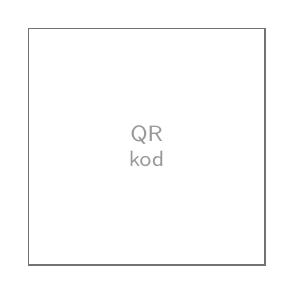
\begin{tikzpicture}
\draw[black!55,line width=0.6pt] (0,0) rectangle (30mm,30mm);
\node[black!40,font=\sffamily\fontsize{8}{9}\selectfont,align=center] at (15mm,15mm) {QR\\kod};
\end{tikzpicture}\\[1.5mm]
{\sffamily\fontsize{9}{11}\selectfont\color{black!70} #1}%
}

\arrayrulecolor{accent}
\setlength{\arrayrulewidth}{0.7pt}
\renewcommand{\arraystretch}{1.35}
\newcommand{\anstitle}[1]{{\sffamily\bfseries\color{accent}\fontsize{11}{13}\selectfont #1}\\[1.3mm]}

\begin{document}

% ================= PAGE 1: Set 1 | Set 2 =================
\topicheader{15}{Statistika Asoslari}
\pagefooter{1}
\colrule{32}{238}
\mbox{}%

\begin{textblock*}{\COLW}(\LCOL,32mm)
{\fontsize{11.5}{14.5}\selectfont
\setkicker{1-to'plam}{Har bir to'plamni tartiblang, so'ng o'rtacha, mediana va modani toping.}

\noindent\pnum{1} $4,\ 8,\ 6,\ 8,\ 2$\\[24mm]
\noindent\pnum{2} $10,\ 12,\ 10,\ 15,\ 13$\\[24mm]
\noindent\pnum{3} $7,\ 9,\ 7,\ 9,\ 7,\ 2$\\[24mm]
\noindent\pnum{4} $1,\ 3,\ 5,\ 7$\\[24mm]
\noindent\pnum{5} $20,\ 22,\ 19,\ 22,\ 18,\ 25$\\[24mm]
\noindent\pnum{6} $6,\ 2,\ 9,\ 2,\ 11$
}
\end{textblock*}

\begin{textblock*}{\COLW}(\RCOL,32mm)
{\fontsize{10.5}{13.5}\selectfont
\setkicker{2-to'plam}{Chastota jadvallari va teskari masalalar.}

\noindent\pnum{1} Ma'lumotlar to'plamida $3$ qiymati ikki marta, $5$ qiymati uch marta va $8$ qiymati bir marta uchraydi. O'rtacha, mediana va modani toping.\\[18mm]
\noindent\pnum{2} $4,7,x,10$ ning o'rtachasi $8$ bo'lsa, $x$ ni toping.\\[16mm]
\noindent\pnum{3} $2,5,9,x,14$ ning o'rtachasi $9$ bo'lsa, $x$ ni toping.\\[16mm]
\noindent\pnum{4} $12,15,12,18,20,15,12$ -- o'rtacha, mediana va modani toping.\\[18mm]
\noindent\pnum{5} $5$ ta sonning o'rtachasi $20$. Ulardan to'rttasi $18,22,19,23$. Beshinchisini toping.\\[16mm]
\noindent\pnum{6} $3,7,x,12,15$ ning mediani $9$ bo'lsa ($x$ -- $7$ va $12$ orasida), $x$ ni toping.
}
\end{textblock*}

\clearpage

% ================= PAGE 2: Set 3 | Set 4 =================
\topicheader{15}{Statistika Asoslari}
\pagefooter{2}
\colrule{32}{238}
\mbox{}%

\begin{textblock*}{\COLW}(\LCOL,32mm)
{\fontsize{10.5}{13.5}\selectfont
\setkicker{3-to'plam}{Guruhlarni to'g'ri birlashtiring -- vaznli o'rtacha, oddiy o'rtacha emas.}

\noindent\pnum{1} A guruh: $10$ kishi, o'rtacha $75$. B guruh: $10$ kishi, o'rtacha $85$.\\[16mm]
\noindent\pnum{2} A guruh: $8$ kishi, o'rtacha $70$. B guruh: $12$ kishi, o'rtacha $90$.\\[16mm]
\noindent\pnum{3} A guruh: $5$ ta, o'rtacha $12$. B guruh: $20$ ta, o'rtacha $20$.\\[16mm]
\noindent\pnum{4} A: $4$ kishi, o'rtacha $60$. B: $6$ kishi, o'rtacha $70$. C: $10$ kishi, o'rtacha $80$.\\[18mm]
\noindent\pnum{5} $30$ talabadan iborat guruhning o'rtachasi $50$. Ichidagi A guruhda $10$ talaba, o'rtacha $40$. Qolgan $20$ talabaning (B) o'rtachasini toping.\\[18mm]
\noindent\pnum{6} A guruhda $6$ talaba, o'rtacha $80$. B guruhda $n$ talaba, o'rtacha $95$. Hammasi $(6+n)$ ning birlashtirilgan o'rtachasi $90$. $n$ ni toping.
}
\end{textblock*}

\begin{textblock*}{\COLW}(\RCOL,32mm)
{\fontsize{10.5}{13.5}\selectfont
\setkicker{4-to'plam}{Chetga chiquvchi (outlier) ta'sirini aniqlang.}

\noindent\pnum{1} $4,5,6,7,8$: o'rtacha va medianani toping. So'ng $50$ qo'shilgandan keyingi yangi o'rtacha va medianani toping. Qaysi ko'rsatkich ko'proq o'zgardi?\\[14mm]
\noindent\pnum{2} $10,12,14,16,18$: o'rtacha va medianani toping. So'ng $-40$ qo'shilgandan keyin qaytadan toping.\\[14mm]
\noindent\pnum{3} $23,45,12,67,34,8$ ning o'zgarish kenglagini (range) toping.\\[14mm]
\noindent\pnum{4} P: $10,12,14,16,18$. Q: $10,12,14,16,100$. Har birining range'ini toping. Qaysi to'plam ko'proq tarqoq?\\[14mm]
\noindent\pnum{5} Agar bitta qiymat juda katta songa almashtirilsa, qaysi markaziy o'lchov (o'rtacha yoki mediana) ko'proq o'zgaradi? Bir gapda sababini tushuntiring.\\[14mm]
\noindent\pnum{6} $15,18,20,19,95,17$: chetga chiquvchi $95$ bilan o'rtachani toping, so'ng uni olib tashlab qaytadan toping.
}
\end{textblock*}

\clearpage

% ================= PAGE 3: Set 5 | Set 6 (spot the error) =================
\topicheader{15}{Statistika Asoslari}
\pagefooter{3}
\colrule{32}{238}
\mbox{}%

\begin{textblock*}{\COLW}(\LCOL,32mm)
{\fontsize{10.5}{13.5}\selectfont
\setkicker{5-to'plam}{Aralash mashqlar -- "Nima so'ralmoqda?" ni diqqat bilan tekshiring.}

\noindent\pnum{1} A guruh: $15$ talaba, o'rtacha $70$. B guruh: $10$ talaba, o'rtacha $x$. Hammasi $25$ talabaning o'rtachasi $76$. $x$ ni toping.\\[16mm]
\noindent\pnum{2} $8,10,12,14$: medianani toping. So'ng $50$ qo'shilgandan keyingi yangi medianani toping.\\[14mm]
\noindent\pnum{3} Test ballari: $70$ (uch talaba), $80$ (besh talaba), $90$ (ikki talaba). O'rtacha va modani toping.\\[14mm]
\noindent\pnum{4} \textbf{Nima so'ralmoqda?} A guruhda $8$ talaba, ballar \emph{yig'indisi} $640$. B guruhda $12$ talaba, o'rtacha $90$. Birlashgan $20$ talabaning ballar \textbf{yig'indisini} toping -- o'rtachasini emas.\\[16mm]
\noindent\pnum{5} \textbf{Nima so'ralmoqda?} $22$ talabaning o'rtacha bali $64$. Ularning ballari \textbf{yig'indisini} toping -- o'rtachani emas.\\[14mm]
\noindent\pnum{6} A guruhda $10$ talaba, ballar yig'indisi $820$. B guruhda $15$ talaba, o'rtacha $88$. Hammasi $25$ talabaning birlashgan o'rtachasini toping. (Diqqat: A guruhning soni yig'indi, o'rtacha emas -- birlashtirishdan oldin aylantiring.)
}
\end{textblock*}

\begin{textblock*}{\COLW}(\RCOL,32mm)
{\fontsize{10.5}{13.5}\selectfont
\setkicker{6-to'plam}{Xatoni toping -- buzilgan qadamni ayting, to'g'ri javobni bering.}

\noindent\pnum{1} Guruh A ning o'rtachasi $60$ ($10$ kishi), Guruh B ning o'rtachasi $80$ ($30$ kishi) haqida ko'rsatilgan yechimda xato bor:\\[1mm]
\hspace*{7mm}\textit{``Birlashtirilgan o'rtacha $=\dfrac{60+80}{2}=70$.''}\\[2mm]
\hspace*{7mm}Xato va to'g'ri javob: \makebox[52mm]{\dotfill}\\[6mm]

\noindent\pnum{2} Ma'lumotlar: $9,2,7,4$ haqida ko'rsatilgan yechimda xato bor:\\[1mm]
\hspace*{7mm}\textit{``Mediana -- qatordagi ikkinchi va uchinchi qiymat, ya'ni $2$ va $7$, demak mediana $=\dfrac{2+7}{2}=4.5$.''}\\[2mm]
\hspace*{7mm}Xato va to'g'ri javob: \makebox[52mm]{\dotfill}\\[6mm]

\noindent\pnum{3} Ma'lumotlar: $3,5,9,11$ haqida ko'rsatilgan yechimda xato bor:\\[1mm]
\hspace*{7mm}\textit{``To'rt qiymat bor, demak mediana -- ikkinchi qiymat, ya'ni $5$.''}\\[2mm]
\hspace*{7mm}Xato va to'g'ri javob: \makebox[52mm]{\dotfill}\\[6mm]

\noindent\pnum{4} Ma'lumotlar: $4,4,6,7,7,7,9$ haqida ko'rsatilgan yechimda xato bor:\\[1mm]
\hspace*{7mm}\textit{``Moda $=4$, chunki u birinchi takrorlangan qiymat.''}\\[2mm]
\hspace*{7mm}Xato va to'g'ri javob: \makebox[52mm]{\dotfill}\\[6mm]

\noindent\pnum{5} Ma'lumotlar: $12,45,8,30$ haqida ko'rsatilgan yechimda xato bor:\\[1mm]
\hspace*{7mm}\textit{``O'zgarish kengligi $=45+8=53$.''}\\[2mm]
\hspace*{7mm}Xato va to'g'ri javob: \makebox[52mm]{\dotfill}
}
\end{textblock*}

\clearpage

% ================= PAGE 4: Set 7 (bonus) =================
\topicheader{15}{Statistika Asoslari}
\pagefooter{4}
\colrule{32}{238}
\mbox{}%

\begin{textblock*}{\COLW}(\LCOL,32mm)
{\fontsize{11}{14}\selectfont
\setkicker{7-to'plam}{Bonus / mastery check -- eng qiyin, ko'p qadamli masalalar.}

\noindent\pnum{1} A guruhda $n$ talaba, o'rtacha $70$. B guruhda $20$ talaba, o'rtacha $85$. Hammasining birlashgan o'rtachasi $80$. $n$ ni toping.\\[30mm]
\noindent\pnum{2} $7$ ta qiymatning o'rtachasi $20$. $8$-qiymat qo'shilib, yangi o'rtacha $22$ bo'ldi. $8$-qiymatni toping.\\[30mm]
\noindent\pnum{3} $19$ talabali sinfning ballar yig'indisi $1425$. Yangi talaba $s$ bali bilan qo'shilib, $20$ talabaning yangi o'rtachasi $73$ bo'ldi. $s$ ni toping.\\[30mm]
\noindent\pnum{4} $5,9,x,20,24$ to'plamining mediani $15$ ($x$ -- tartiblangandan keyin $3$-o'rinda). $x=15$ izchilligini tasdiqlang (ya'ni u $9$ va $20$ orasida joylashishini) va bu tekshiruv nima uchun muhimligini tushuntiring.\\[18mm]
\noindent\pnum{5} A: $10$ talaba, o'rtacha $60$. B: $n$ talaba, o'rtacha $90$. C: $6$ talaba, o'rtacha $70$. Hammasi $(10+n+6)$ ning birlashgan o'rtachasi $78$. $n$ ni toping.
}
\end{textblock*}

\clearpage

% ================= PAGE 5: Javoblar -- full-page unified answer table + QR =================
\topicheader{15}{Statistika Asoslari}
\pagefooter{5}
\mbox{}%

\begin{textblock*}{194mm}(16mm,30mm)
{\bfseries\itshape\color{accent}\fontsize{19}{21}\selectfont\centering Javoblar\par}
\end{textblock*}

\begin{textblock*}{194mm}(16mm,40mm)
{\fontsize{7.6}{9.3}\selectfont
\centering
\renewcommand{\arraystretch}{1.0}
\begin{tabular}{|>{\centering\arraybackslash}p{22mm}|>{\centering\arraybackslash}p{7mm}|>{\raggedright\arraybackslash}p{150mm}|}
\hline
\rowcolor{badge!55}\textbf{To'plam} & \textbf{\#} & \textbf{Javob}\\
\hline
\multirow{6}{22mm}{\centering 1-to'plam} & 1 & mean $=\frac{28}{5}=5.6$, median $=6$, mode $=8$\\\cline{2-3}
 & 2 & mean $=12$, median $=12$, mode $=10$\\\cline{2-3}
 & 3 & mean $=\frac{41}{6}$, median $=7$, mode $=7$\\\cline{2-3}
 & 4 & mean $=4$, median $=4$, mode $=$ yo'q (barcha qiymat bir marta)\\\cline{2-3}
 & 5 & mean $=21$, median $=21$, mode $=22$\\\cline{2-3}
 & 6 & mean $=6$, median $=6$, mode $=2$\\\hline
\multirow{6}{22mm}{\centering 2-to'plam} & 1 & mean $=\frac{29}{6}$, median $=5$, mode $=5$\\\cline{2-3}
 & 2 & $x=11$\\\cline{2-3}
 & 3 & $x=15$\\\cline{2-3}
 & 4 & mean $=\frac{104}{7}$, median $=15$, mode $=12$\\\cline{2-3}
 & 5 & beshinchi son $=18$\\\cline{2-3}
 & 6 & $x=9$\\\hline
\multirow{6}{22mm}{\centering 3-to'plam} & 1 & $80$\\\cline{2-3}
 & 2 & $82$\\\cline{2-3}
 & 3 & $\frac{92}{5}=18.4$\\\cline{2-3}
 & 4 & $73$\\\cline{2-3}
 & 5 & $55$\\\cline{2-3}
 & 6 & $n=12$\\\hline
\multirow{6}{22mm}{\centering 4-to'plam} & 1 & Boshida: mean$=6$, median$=6$. $50$dan keyin: mean$\approx13.33$, median$=6.5$. \textbf{Mean ko'proq o'zgardi.}\\\cline{2-3}
 & 2 & Boshida: mean$=14$, median$=14$. $-40$dan keyin: mean$=5$, median$=13$. \textbf{Mean ko'proq o'zgardi.}\\\cline{2-3}
 & 3 & range $=67-8=59$\\\cline{2-3}
 & 4 & range P$=8$; range Q$=90$. \textbf{Q ko'proq tarqoq.}\\\cline{2-3}
 & 5 & Mean -- har bir qiymatning aniq kattaligiga bog'liq, shu sabab bitta chetga chiquvchi uni kuchli tortadi; mediana faqat tartibdagi o'ringa bog'liq.\\\cline{2-3}
 & 6 & Chetga chiquvchi bilan: mean$\approx30.67$. Usiz: mean$=17.8$.\\\hline
\multirow{6}{22mm}{\centering 5-to'plam} & 1 & $x=85$\\\cline{2-3}
 & 2 & median$=11$; $50$ qo'shilgach median$=12$\\\cline{2-3}
 & 3 & mean$=79$, mode$=80$\\\cline{2-3}
 & 4 & yig'indi $=640+12\times90=1720$\\\cline{2-3}
 & 5 & yig'indi $=22\times64=1408$\\\cline{2-3}
 & 6 & A mean$=82$; birlashgan mean$=\frac{820+15\times88}{25}=85.6$\\\hline
\multirow{5}{22mm}{\centering 6-to'plam} & 1 & Xato -- guruh o'lchamlarini (10 vs 30) hisobga olmay o'rtachalarni to'g'ridan-to'g'ri o'rtachalagan. To'g'ri: $\frac{10\times60+30\times80}{40}=75$.\\\cline{2-3}
 & 2 & Xato -- tartiblanmagan ro'yxatdan mediana olingan. Tartiblangan: $2,4,7,9$; mediana$=\frac{4+7}{2}=5.5$.\\\cline{2-3}
 & 3 & Xato -- juft sondagi to'plam uchun o'rtadagi o'rinni noto'g'ri hisoblagan. Mediana$=\frac{5+9}{2}=7$.\\\cline{2-3}
 & 4 & Xato -- birinchi ko'ringan takroriy qiymatni moda deb atagan. To'g'ri moda$=7$ (uch marta takrorlangan).\\\cline{2-3}
 & 5 & Xato -- range'ni yig'indi sifatida hisoblagan. To'g'ri: $45-8=37$.\\\hline
\multirow{5}{22mm}{\centering 7-to'plam} & 1 & $n=10$\\\cline{2-3}
 & 2 & 8-qiymat$=22\times8-20\times7=36$\\\cline{2-3}
 & 3 & $s=73\times20-1425=35$\\\cline{2-3}
 & 4 & $x=15$ izchil, chunki $9\le15\le20$.\\\cline{2-3}
 & 5 & $n=19$\\\hline
\end{tabular}
}
\end{textblock*}

\begin{textblock*}{194mm}(16mm,238mm)
\centering
{\sffamily\fontsize{9.5}{11.5}\selectfont\color{black!70} Video yechimlar va qo'shimcha testlar uchun quyidagi QR kodlarni skanerlang:}\\[4mm]
\begin{minipage}[t]{32mm}\centering\qrbox{YouTube}\end{minipage}%
\hspace{16mm}%
\begin{minipage}[t]{32mm}\centering\qrbox{Telegram}\end{minipage}
\end{textblock*}

\end{document}
